\documentclass{article}
\usepackage{geometry}
\geometry{
	a4paper,
	%total={170mm,257mm},
	left=20mm,
	top=30mm,
}

\usepackage{fancyhdr}
\usepackage{tikz}
\usepackage{hyperref}
\usepackage{graphicx}
\usepackage{hyperref}
\usepackage{mdframed}
\usepackage{listings} % Include the listings package
\usepackage{xcolor}   % to define your own colors

\bibliographystyle{unsrt}
\bibliography{references}


\newmdenv[
linecolor=blue, % Color of the border line
backgroundcolor=gray!20, % Background color; "gray!20" means "20% gray"
frametitle=Note, % Title of the frame, delete this line if you don't want a title
skipabove=\baselineskip, % Space above the frame
skipbelow=\baselineskip, % Space below the frame
]{mynote}

% code-snippets:
% Define the color styles you wish to use in the document for the Python syntax highlighting
\lstdefinestyle{mystyle}{
	backgroundcolor=\color{white},   % choose the background color; you must add \usepackage{color} or \usepackage{xcolor}
	commentstyle=\color{green},
	keywordstyle=\color{blue},
	numberstyle=\tiny\color{gray},
	stringstyle=\color{red},
	basicstyle=\ttfamily\footnotesize,
	breakatwhitespace=false,         
	breaklines=true,                 
	captionpos=b,                    
	keepspaces=true,                 
	numbers=left,                    
	numbersep=5pt,                  
	showspaces=false,                
	showstringspaces=false,
	showtabs=false,                  
	tabsize=2
}

\lstset{style=mystyle} % Apply your style globally to the document


\newcommand{\LVA}{Reverse Engineering}
\newcommand{\LVAKURZ}{REV3}
\newcommand{\SEMESTER}{WS 2023/2024}
\newcommand{\UELABEL}{UE 01}
\newcommand{\UETITLE}{Schutzmechanismen}
\newcommand{\AUTHOR}{Jakob Mayr}


\title{\vspace{5cm} \LVA\ (\LVAKURZ)\\ \vspace{1cm} \textbf{\UELABEL\ -- \UETITLE\ -- Protokoll} \vspace{2.5cm}}
\author{\AUTHOR}
\date{\SEMESTER}

\begin{document}
	
	\pagestyle{fancy}
	
	\maketitle
	
	\tikz [remember picture, overlay] %
	\node [shift={(3.7cm,-4cm)}] at (current page.north west) %
	[anchor=north west] %
	{
\includegraphics{fhooe_logo.jpg}};
	
	\tikz [remember picture, overlay] %
	\node [shift={(10cm,-4.8cm)}] at (current page.north west) %
	[anchor=north west] %
	{
\includegraphics{si_logo.jpg}};
	
	%\tikz [remember picture, overlay] %
	%\node [shift={(7.2cm,-11.65cm)}] at (current page.north west) %
	%[anchor=north west] %
	%{\includegraphics[scale=0.12]{./img/star_wars_logo_no_background.png}};
	%
	%\pagebreak
	
	\fancyhf{}
	\fancyhead[L]{\LVA\ (\LVAKURZ)}
	\fancyhead[C]{\UELABEL}
	\fancyhead[R]{\SEMESTER}
	\fancyfoot[L]{Seite \thepage\ von \pageref{LastPage}}
	\fancyfoot[R]{\AUTHOR}
	
	\section{Einleitung}
	Folglich werden 4 Files "hello[1-4].exe", analysiert, deren Schutz "geknackt" und verändert, sodass sie "SIB22" anstatt "Hello" ausgeben.\\
	Zu erzielende Ausgabe:\\
	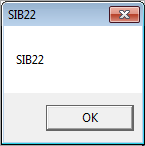
\includegraphics[width=0.25\linewidth]{pictures/SIB22}		
	
	\pagebreak
	
	\section{Verschlüsselung/Komprimierung}
	\subsection{hello1.exe}
	Das PE-File "hello1.exe" verwendet für die "Entschlüsselung" eine XOR-Operation über einen Addressbereich im Datensegment.\\
	Das EBX-Register stellt für die "Entschlüsselung" den Zähler dar (Adressbereich wird von größter zu kleinster Adresse durchiteriert). Die Startadresse (401017) + "Wert im EBX-Register" zeigt auf das jeweilige zu entschlüsselnde Byte und durch das dekrementieren des EBX-Registers werden all 33 Bytes "entschlüsselt".\\
	Der "Schlüssel" für das XOR ist 0x96 (im ECX Register).\\
	Codesnipped für XOR-Entschlüsselung:\\
	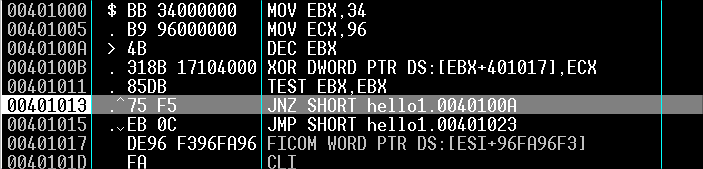
\includegraphics[width=0.5\linewidth]{pictures/hello1-important code-snipped}\\
	Die Addresse für dieses Datensegment kann in "OllyDbg" via der Option "Follow in Dump/Selection" angezeigt werden.\\
	\("Hello" \oplus 0x96\) ergibt folgenden Wert:\\
	\texttt{de 96 f3 96 fa 96 fa 96 f9 96}\\
	\\
	Dieser Wert kann auch in einem Hex-Editor gefunden werden. Durch ersetzen mit \("SIB22" \oplus 0x96\) kann ein neues File erstellt werden welches "SIB22" im Fenster anzeigt.\\
	\("Hello" \oplus 0x96\) ergibt folgenden Wert:\\
	\texttt{c5 96 df 96 d4 96 a4 96 a4 96}\\
	
	\subsection{hello2.exe}
	Das zweite PE-File "hello2.exe" arbeitet sehr ähnlich wie "hello1.exe", mit dem Unterschied, dass im Addressbereich in die andere Richtung entschlüsselt wird (Adresse erhöht sich nun) und dass nicht Byte-weise sonder immer 4-Byte-weise oder jeweils ein DWORD (32-bit) entschlüsselt wird.\\
	Codesnipped für XOR-Entschlüsselung:\\
	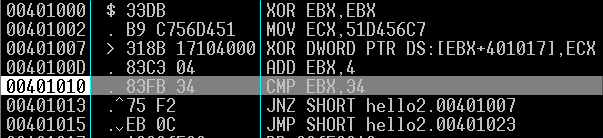
\includegraphics[width=0.5\linewidth]{pictures/hello2-important-code-snipped}\\
	Der Key hierbei muss natürlich auch 32-Bit haben:\\
	\texttt{C7 56 D4 51}\\
	"Hello" in verschlüsselter Form hat folgende Form:\\
	\texttt{8F 56 B1 51 AB 56 B8 51 A8 56}\\
	"SIB22" in verschlüsselter Form hätte hierbei folgende Form:\\
	\texttt{94 56 9d 51 85 56 e6 51 f5 56}\\
	
	\begin{mynote}
		Hierbei sehr aufällig ist, dass das Padding der Buchstaben (0x00) sich mit dem Schlüssel deckt, deshalb wiederholt sich "0x56" und "0x51" immer wieder.
	\end{mynote}
	
	\pagebreak
	
	\subsection{hello3.exe}
	Auch das PE-File "hello3.exe" arbeit sehr ähnlich. Hierbei wird der Adressbereich jedoch zweimal "ge-xor'd". Einmal mit einem statischen Wert "0x69" und einmal mit dem Wert aus dem EBX-Register welches auch gleichzeitig wieder den Zähler darstellt. (Hierbei wird die Adresse wieder vermindert)\\
	Einfach erklärt wird die das Byte an der höchsten Adresse wie folgt entschlüsselt:\\
	\("5B" \oplus 0x69 \oplus 0x32\)\\
	Das folgenden Bytes werden dann wie folgt entschlüsselt:\\
	\("18" \oplus 0x69 \oplus 0x31\)\\
	\("79" \oplus 0x69 \oplus 0x30\)\\
	...\\
	Da dies händlisch ein wenig aufwendig ist, kann die auch via Python realisiert werden ():
	\begin{lstlisting}[language=Python]
		def xor_process(hex_data):
			xor_value = 0x69
			decrementing_value = 0x32
			
			result = []
			
			for byte in hex_data:
			# XOR with 0x69 and the decrementing value
			xor_result = byte ^ xor_value ^ decrementing_value
			
			print(f"input_byte: {hex(byte)}\ndecrementing_value: {hex(decrementing_value)}\nxor_result{hex(xor_result)}\tascii: {chr(xor_result)}\n")
			result.append(xor_result)
			
			if decrementing_value == 0:
			print("end of decrementing")
			break
			decrementing_value -= 1
			
			return result
		
		# Input data (hexadecimal bytes)
		hex_str_hello = (
		"BB 33 00 00 00 B9 69 00 00 00 03 C3 4B 31 8B 1F 10 40 00 31 9B 1F 10 40 00 85 DB 75 EF EB 0C 21 68 0E 6A 01 6C 03 6E 0E 60 63 62 0F 64 0F 79 69 38 7B 12 62 6C 3F 7E 1B 70 9B 7C 75 75 77 1C 49 A0 4A 4A 4D 4C 83 B1 64 40 63 02 45 BB 62 4E 79 18 5B"
		)
		
		hex_str_sib = (
		"BB 33 00 00 00 B9 69 00 00 00 03 C3 4B 31 8B 1F 10 40 00 31 9B 1F 10 40 00 85 DB 75 EF EB 0C 3a 68 22 6A 2F 6C 5D 6E 53 60 63 62 0F 64 0F 79 69 38 7B 12 62 6C 3F 7E 1B 70 9B 7C 75 75 77 1C 49 A0 4A 4A 4D 4C 83 B1 64 40 63 02 45 BB 62 4E 79 18 5B"
		)
		
		print("------------ Hello part ------------")
		hex_bytes_hello = [int(h, 16) for h in hex_str_hello.split()]
		hex_bytes_hello = [int(h, 16) for h in hex_str_hello.split()]
		
		processed_bytes_hello = xor_process(hex_bytes_hello[::-1])
		processed_hex_hello = ['{:02X}'.format(b) for b in processed_bytes_hello]
		print(' '.join(processed_hex_hello))
		
		print("------------ SIB part ------------")
		
		hex_bytes_sib = [int(h, 16) for h in hex_str_sib.split()]
		hex_bytes_sib = [int(h, 16) for h in hex_str_sib.split()]
		
		processed_bytes_sib = xor_process(hex_bytes_sib[::-1])
		processed_hex_sib = ['{:02X}'.format(b) for b in processed_bytes_sib]
		print(' '.join(processed_hex_sib))
	\end{lstlisting}
	
	\pagebreak
	
	Codesnipped für XOR-Entschlüsselung:\\
	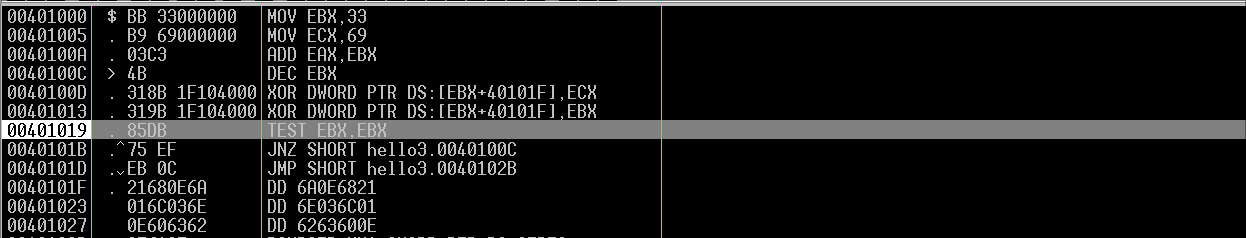
\includegraphics[width=0.5\linewidth]{pictures/hello3-important-code-snipped}\\
	\begin{mynote}
		Der Teil der hierbei in Python entschlüsselt wird ist natürlich länger als das eigentliche Python, es müssen wieder nur 5 Bytes geändert werden:\\
		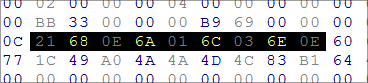
\includegraphics[width=0.5\linewidth]{pictures/hello3-hex editor}\\
	\end{mynote}
	
	\subsection{hello4.exe}
	Das "hello4.exe" PE-File verwendet keine Verschlüsselung sondern eine Komprimierung. Deaktiviert man das Plugin "UPX Unpacker Plug-in" im PE-Explorer und öffnet das File, so sieht man, dass die "Section-Headers" untypisch "UPX0", "UPX1" und "UPX2" heißen. Ebenfalls erkennt man z.b., dass die UPX0 eine "Size of Raw Data" von 0 hat, aber eine "Virtual Size" von 4000. Durch diese Dinge kann man bereits darauf schließen, dass das PE-File mit UPX (Ultimate Packer for Executables) kompriemiert wurde.\\
	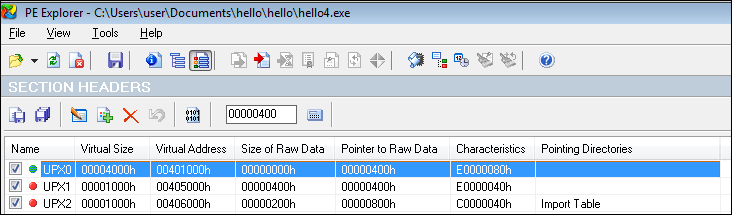
\includegraphics[width=0.5\linewidth]{pictures/UPX-section headers (no plugin)}\\
	UPX Unpacker Plug-in:\\
	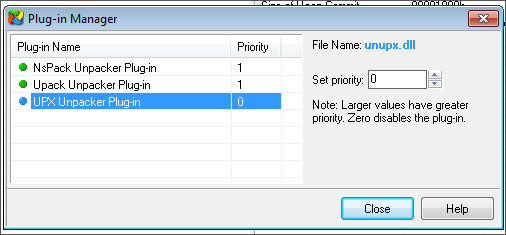
\includegraphics[width=0.5\linewidth]{pictures/hello4-upx-plugin pe-explorer}\\
	Aktiviert man nun das Plugin, öffnet das File und speichert es "entpackt" (entpackt sich beim öffnen), dann hat man wieder ein "normales" PE-File. Anschließend kann in einem Hex-Editor der Hex-Wert für "Hello" (\texttt{48 65 6c 6c 6f, bzw 48 00 65 00 6c 00 6c 00 6f 00}) gesucht und durch den Hex-Wert für "SIB22" (\texttt{53 49 42 32 32, bzw 53 00 49 00 42 00 32 00 32 00}) ersetzt werden.\\
	Folglich ein Screenshot der Stelle im Hex-Editor, welche "SIB22" zeigt.\\
	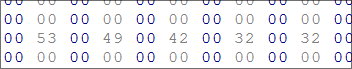
\includegraphics[width=0.5\linewidth]{pictures/hello4-after unpacking edit in hex-explorer}\\
	
	\pagebreak
	
	\section{Radare2}
	\subsection{hello1.exe}
	Folgender Aufruf von Radare2 zeigt den code an der Einsprungsaddresse von hello1.exe und damit auch die Instruktionen für das entschlüsseln:\\
	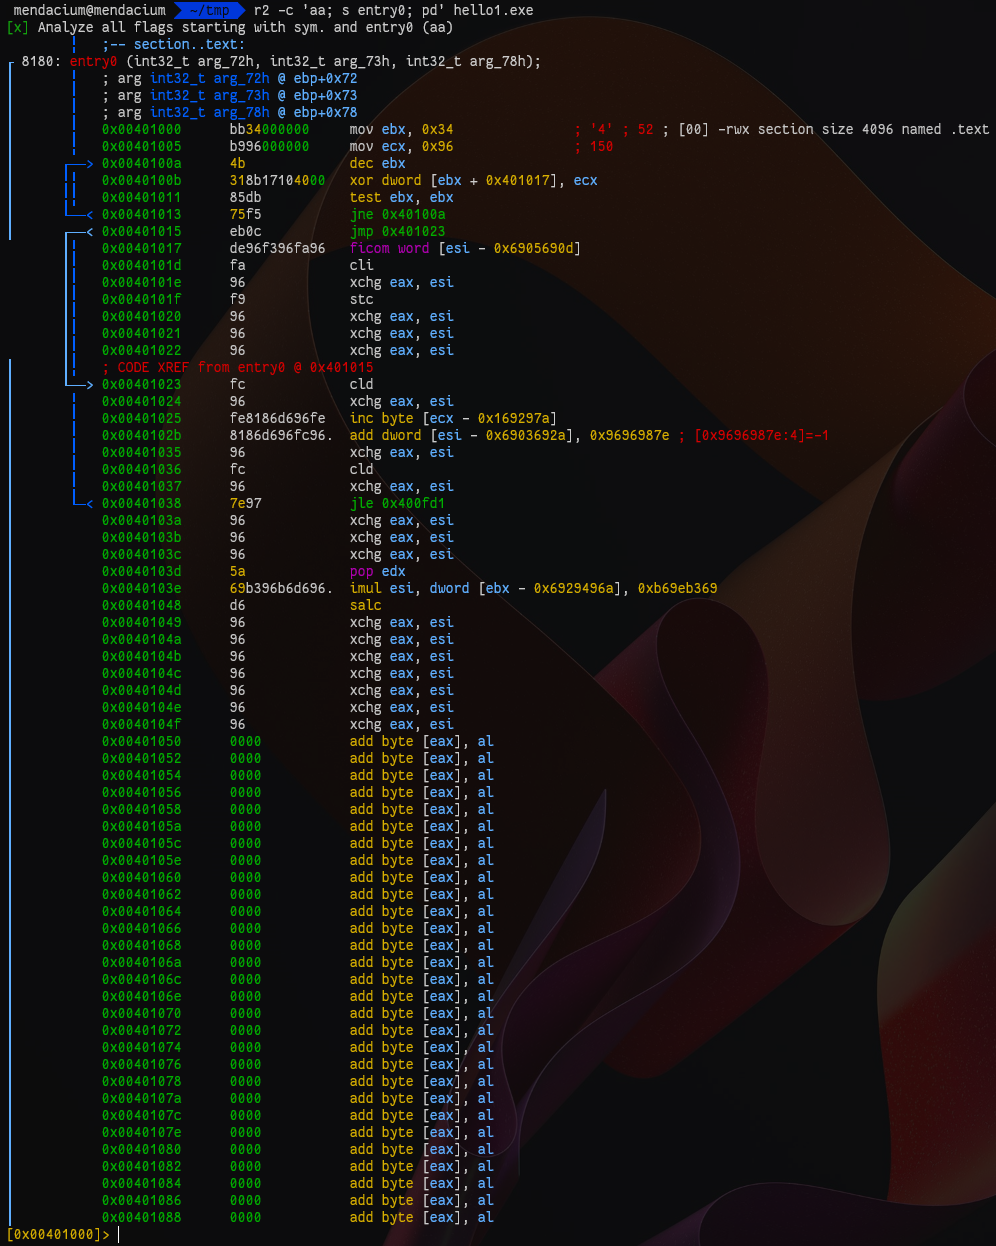
\includegraphics[width=0.5\linewidth]{pictures/hello1-radare2}\\
	
	\subsection{hello2.exe}
	Folgender Aufruf von Radare2 zeigt den code an der Einsprungsaddresse von hello2.exe und damit auch die Instruktionen für das entschlüsseln:\\
	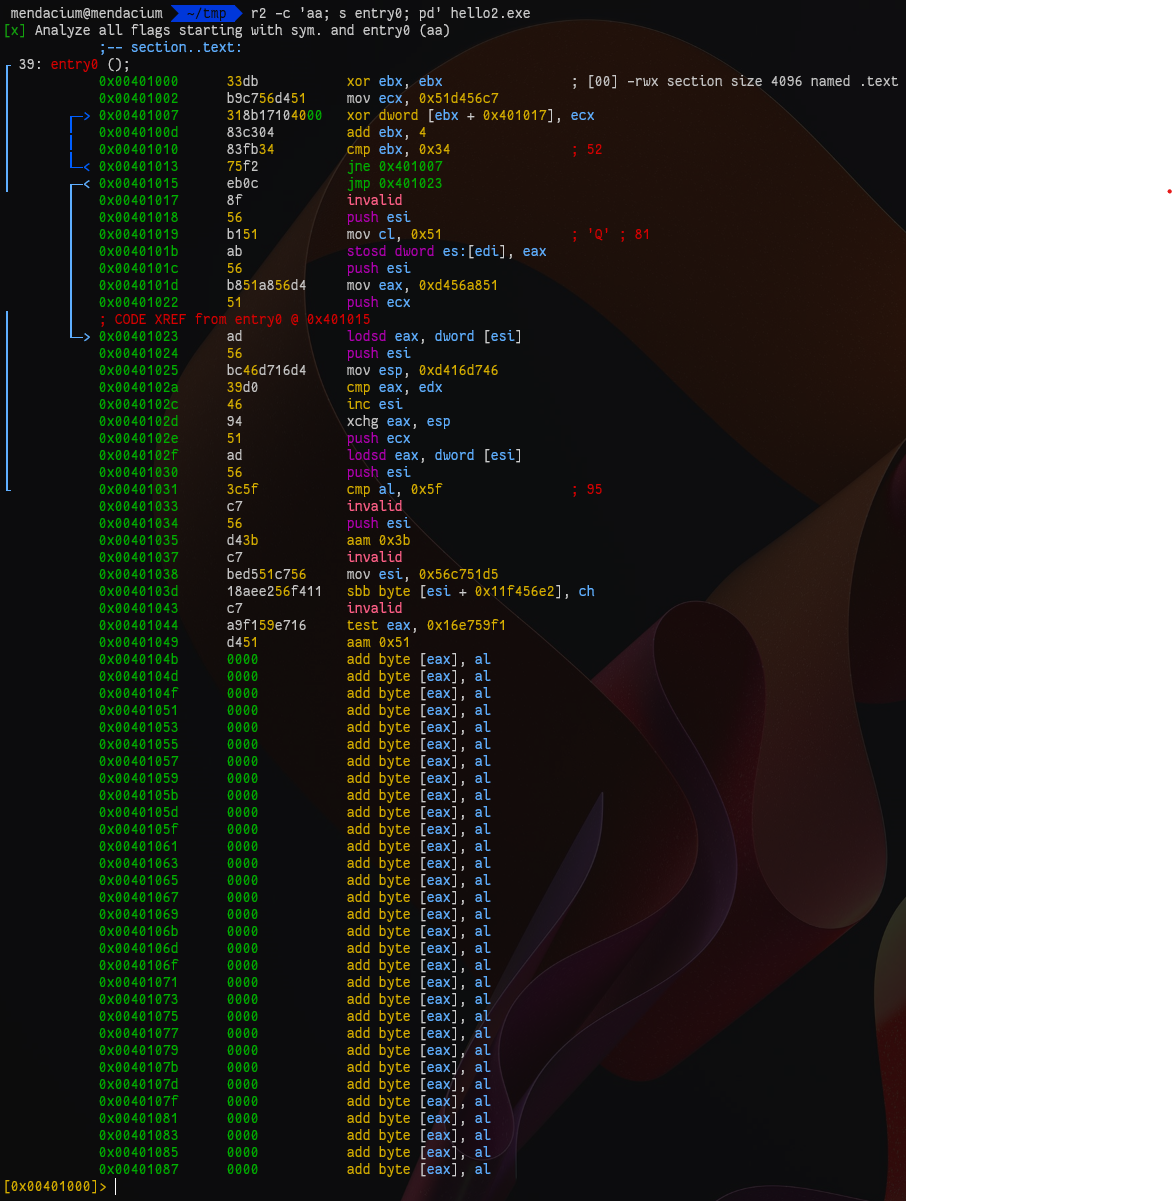
\includegraphics[width=0.5\linewidth]{pictures/hello2-radare2}\\
	
	\subsection{hello3.exe}
	Folgender Aufruf von Radare2 zeigt den code an der Einsprungsaddresse von hello3.exe und damit auch die Instruktionen für das entschlüsseln:\\
	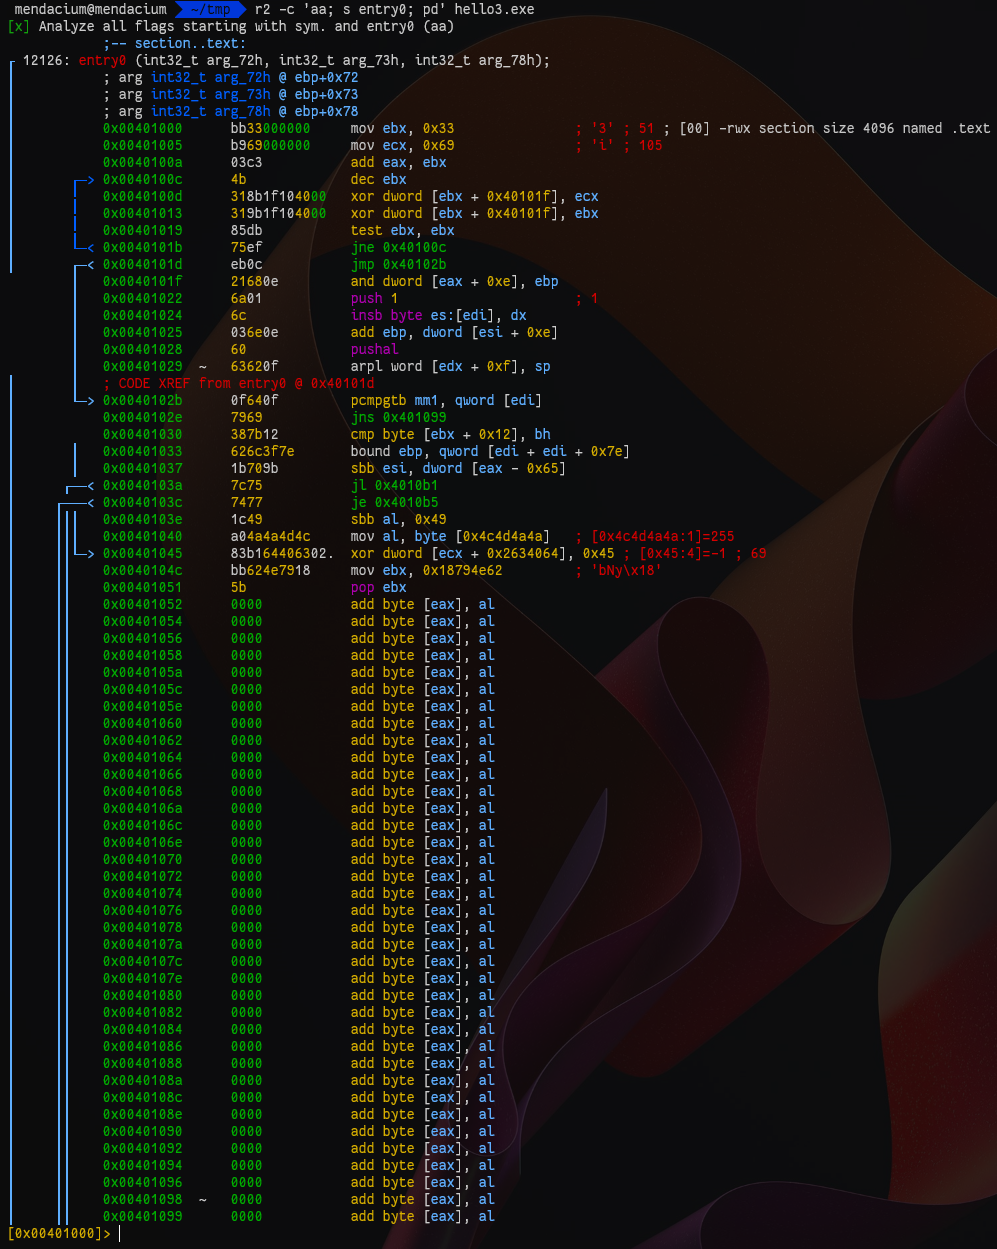
\includegraphics[width=0.5\linewidth]{pictures/hello3-radare2}\\
	
	\pagebreak
	
	\subsection{hello4.exe}
	Da im PE-File "hello4.exe" keine Entschlüsselung wie in den Beispielen zuvor durchgeführt wird, kann etwas anderes angezeigt werden.\\
	Das PE-File kann auch via CommandLine entpackt werden und anschließend kann in radare2 nach dem Hex-Wert für "Hello" gesucht werden und dieser ausgegeben werden:\cite{radare2}\\
	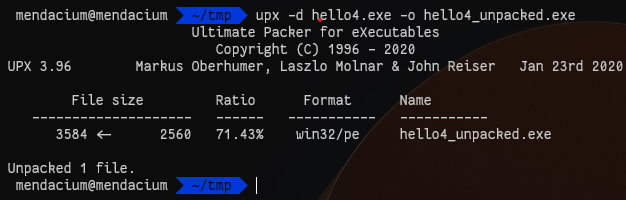
\includegraphics[width=0.5\linewidth]{pictures/hello4-upx-decompress}
	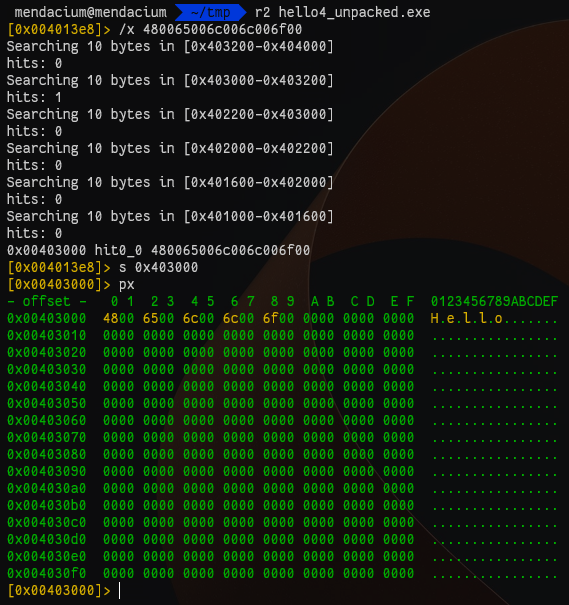
\includegraphics[width=0.5\linewidth]{pictures/hello4-radare2}\\
	
	\begin{thebibliography}{9}
		
		\bibitem{radare2}
		\emph{The Official Radare2 Book},
		[Online; abgerufen im Oktober 2023],
		\url{https://book.rada.re/}.
		
	\end{thebibliography}
	
	
	\label{LastPage}
	
\end{document}